\documentclass[a4paper,10pt]{article}
\usepackage{geometry}
\usepackage{tcolorbox}
\usepackage{listings}
\usepackage[table]{xcolor}
\usepackage{amsmath}
\usepackage{graphicx}
\usepackage{wrapfig}
\usepackage{hyperref}
\usepackage{enumitem}
\usepackage{multicol}
\usepackage{tikz}
\usepackage{array}
% \usepackage{paralist}

\geometry{
    top=1.2cm,
    bottom=1.5cm,
    left=1.3cm,
    right=1.3cm
}

\definecolor{codegray}{rgb}{0.9,0.9,0.9}
\definecolor{darkblue}{rgb}{0,0,0.5}

\setlength{\tabcolsep}{2pt}

\lstdefinestyle{mystyle}{
    backgroundcolor=\color{codegray},   
    commentstyle=\color{darkblue},
    keywordstyle=\color{blue},
    numberstyle=\tiny\color{gray},
    stringstyle=\color{red},
    basicstyle=\ttfamily\footnotesize,
    breaklines=true,
    numbers=left,                    
    numbersep=5pt,                  
    showspaces=false,                
    showstringspaces=false,
    showtabs=false,                  
    tabsize=4
}
\lstset{style=mystyle}
\newtcolorbox{definitionbox}[1]{colback=blue!5!white,colframe=blue!75!black,title=#1}
\hypersetup{
    colorlinks=true,
    linkcolor=blue,
    filecolor=magenta,      
    urlcolor=blue,
}
\setlist[itemize]{nosep}

\newcommand{\hl}[1]{\textcolor{violet}{\textit{#1}}}
\renewcommand{\arraystretch}{0.8}
\newcommand{\tabletitle}[1]{\multicolumn{2}{c}{\textbf{#1}}}

\title{\huge Laborator Arhitectura Sistemelor de Calcul - FMI}
\author{
  Matei-Iulian Cocu\\
  \texttt{matei-iulian.cocu@s.unibuc.ro}
  \and
  Ștefan Chiper\\
  \texttt{stefan.chiper@s.unibuc.ro}
} \date{}
\renewcommand*\contentsname{\large\bfseries Cuprins}

\begin{document}
\maketitle
\setcounter{tocdepth}{2}
\tableofcontents
\thispagestyle{empty}
\newpage

\section{Laborator 0x00: Introducere în limbajul de programare Assembly x86}
\subsection{Introducere}
Scopul acestui laborator este acela de a va introduce limbajul Assembly x86 si de a va obisnui cu
sintaxa AT\&T pentru procesoarele x86. In acest sens, accentul este pus, in mare parte, pe insusirea
notiunilor elementare de programare intr-un limbaj de asamblare.


\subsection{Masina virtuala \& Git}
\subsubsection{Masina virtuala / Windows subsystem for Linux}
Acest laborator va fi predat sub Linux, astfel ca daca nu aveti o distributie de Linux ca sistem
principal de operare, va trebui sa va instalati cel putin pe o masina virtuala. Recomandarea este sa
va luati o imagine de Ubuntu si sa o instalati pe VMWare sau pe VirtualBox. 
Imaginea sistemului de operare o gasiti pe site-ul de la \href{https://ubuntu.com/download/desktop}{Ubuntu}.
Doua tutoriale video excelente pentru instalarea mediului de lucru, impreuna cu unele sugestii de setare
pentru sistem le gasiti aici: 
\begin{itemize}
    \item Windows \& Ubuntu (other Linux-based - Debian) OS: \url{https://youtu.be/XGr6_QV5moU}
    \item MacOS Apple Silicon (Mx Normal/Pro/Max): \url{https://youtu.be/1kENnRk39J0}
\end{itemize}
Daca nu ati mai folosit Linux, o investitie buna pentru viitorul
vostru este un alt \href{https://www.youtube.com/watch?v=wBp0Rb-ZJak}{tutorial} putin mai detaliat.

\subsubsection{Git}
La aceast curs, tot codul sursa scris de voi va fi integrat intr-un sistem pentru controlul versiunilor.
Aceasta este o practica standard in industria software. Munca din timpul laboratoarelor va fi salvata
pe Git. In acest sens, va recomand sa va faceti un cont pe Github, sa va creati un repository cu
numele ”Laborator ASC” sau similar, iar toate problemele pe care le lucrati sa le aveti centralizate
aici. Cand/daca aveti intrebari legate de programele realizate la acest laborator noi le putem verifica
direct online pe Git si va putem sugera solutii. \\
Un \href{https://www.youtube.com/playlist?list=PL4cUxeGkcC9goXbgTDQ0n_4TBzOO0ocPR}{tutorial} video excelent pentru instalarea Git pe sistemul vostru este disponibil online.

\subsection{Limbajul Assembly x86}
Assembly x86 este un limbaj de programare de nivel scazut (low-level programming language)
care permite controlul direct asupra unitatii centrale de calcul (CPU) a unui calculator cu arhitectura
de calcul x86. In multe limbaje de programare de nivel inalt compilatorul creeaza prima data cod
assembly ca un pas intermediar. Codul sursa assembly este o bucata de text, deci un procesor nu are
cum sa interpreteze si sa execute acest text. Assembly este transformat apoi in cod masina (machine
code): instructiuni masina binare codate clar (opcode) care pot fi apoi executate de procesor pas
cu pas. Vrem sa va atragem atentia ca Assembly x86 are doua sintaxe distincte: Intel (folosit pe
sisteme Windows) si AT\&T (folosit predominant pe sisteme Unix). In acest laborator folosim doar sintaxa AT\&T. Daca intelegeti una dintre sintaxe, cealalta e foarte usor
de citit si inteles.
Componentele principale ale limbajului Assembly x86 sunt:
\begin{itemize}
    \item Registrii. Ca in orice limbaj de programare, avem nevoie de variable cu care sa lucram. Aceste
variable stocheaza date (in cazul nostru, valori pe 32 biti). Putem seta si modifica valorile
registrilor si putem realiza operatii cu si intre acesti registri (de exemplu: putem aduna valorile
din doi registri si il putem pune intr-un al treilea, sau in unul dintre registrii care deja stocheaza
un operand). Unii registri stocheaza o locatie in memorie (de exemplu: trebuie sa stim unde
se afla urmatoarea instructiune din program care trebuie executata, deci avem un Instruction
Pointer - e defapt un “Instruction Register”);
    \item Instructiuni. Procesorul suporta o serie de operatii intre registrii si locatii din memorie. In
primul rand avem nevoie de abilitatea de a muta din/in registri date in/din memorie. In
registri, putem face operatii matematice, logice, I/O, etc.
    \item Flaguri. Dupa ce facem o operatie, avem o serie de flag-uri (indicatori) care se activeaza in
functie de rezultat (daca rezultatul operatilor este negativ sau zero, sau daca un overflow s-a
produs);
    \item  Adresarea memoriei. In procesor avem doar cativa registri. Daca avem nevoie sa lucram cu un
volum mare de date (de exemplu, continutul unui fisier) atunci avem nevoie sa ne putem referi
la o adresa din memorie (Random Access Memory - RAM ). Accesul la registri este rapid, dar
citirea/scrierea datelor din/in RAM este o operatie mult mai lenta ca timp;
    \item Stiva programului. Orice program care se afla in executie are o locatie speciala de memorie
care se numeste stiva (the program stack). Aceasta este o structura de date de tip Last In First
Out (LIFO). Vom vedea mai tarziu exemple unde aceasta structura este folositoare (apelul de
functii in Assembly);
    \item Intreruperi. Programul pe care voi il executati (indiferent de limbajul de programare) nu
are acces direct la toate resursele hardware. In cele mai multe cazuri, sistemul de operare
controleaza accesul la memorie si periferice. De aceea, avem nevoie sa cerem sistemului de
operare sa execute niste operatii pentru programul nostru. Aceasta delegare a muncii catre
sistemul de operare se realizeaza prin intreruperi.
\end{itemize}
\vspace{50pt}
\subsection{Registrii}
\begin{wrapfigure}{r}{0.48\textwidth}
    \vspace{-25pt}
    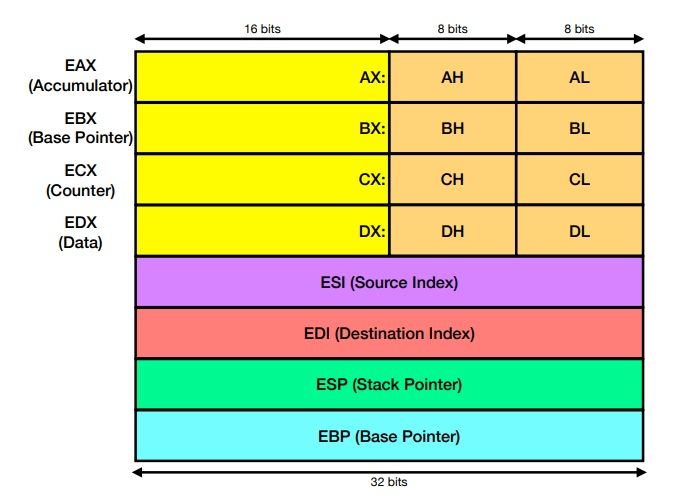
\includegraphics[width=0.45\textwidth]{../resources/registrii.jpg}
    \caption{Registrii x86}
\end{wrapfigure}
Arhitectura procesorului este pe 32 de biti, 
astfel ca registrii utilizati sunt tot pe 32 de biti. Un
registru reprezinta o cantitate mica de spatiu de stocare pe unitatea centrala de procesare, al carui
continut poate fi accesat mai rapid decat datele stocate in alt loc (de exemplu, in memorie sau chiar
mai lent pe hard-disk). \\
Registrii arhitecturii x86 sunt:
\begin{itemize}
    \item cei 8 din imaginea de mai sus, numiti registrii de uz general (General-Purpose Registers);
    \item un registru pentru flags;
    \item un registru pointer la instructiunea urmatoare ce va fi executata (Instruction Pointer);
    \item alti registrii
\end{itemize}
\vspace{5pt}
\textbf{Observatie}: Registrul \textbf{BP} poate fi utilizat si ca frame pointer. \\
\textbf{Alta observatie}: Urmarim tabelul si observam ca registrii pe arhitectura x86 pe 32 de biti au
prefixul \textbf{E} (extended). In acest caz, registrul \textbf{EAX} este format din \textbf{AX} (accumulator), \textbf{AH} (H - high) si \textbf{AL} (L
- low). De exemplu, daca in \textbf{EAX} stocam valorea 0, dar punem in \textbf{AH} ulterior valoarea 1, atunci
intreg registrul \textbf{EAX} va stoca valoarea 256 in baza 10.




\section{Laborator 0x01: Probleme avansate în Assembly x86}
\subsection{}

\subsection{}

\subsection{}

\subsection{Lectură suplimentară}

\section{Laborator 0x02: Introducere în RISC-V}
\subsection{}

\subsection{}

\subsection{}

\subsection{Lectură suplimentară}

\end{document}